% Copyright 2021 Joel Feldman, Andrew Rechnitzer and Elyse Yeager, except where noted.
% This work is licensed under a Creative Commons Attribution-NonCommercial-ShareAlike 4.0 International License.
% https://creativecommons.org/licenses/by-nc-sa/4.0/


\begin{frame}{Table of Contents}

\mapofcontentsC{\ce}
\end{frame}

%----------------------------------------------------------------------------------------
%----------------------------------------------------------------------------------------
%----------------------------------------------------------------------------------------
\section{3.5: Optimisation}
%----------------------------------------------------------------------------------------
%----------------------------------------------------------------------------------------
%-------------------------------------------------------------
\begin{frame}
Optimisation:\\
finding the biggest/smallest/highest/lowest, etc.\pause
\vfill
Lots of non-standard problems! Opportunities to work on your problem-solving skills.
\end{frame}
%-----------------------------
\note{We start with some problems that someone might want to solve, only by way of motivation. We won't actually solve them here.}
%-----------------------------

\begin{frame}{Engineering Design Example}
A lever of density 3 lbs/ft is being used to lift a 500-pound weight, attached one foot from the fixed point.
\begin{center}
\vspace{-1em}
	\begin{tikzpicture}
	\draw(0,0)node[vertex](fulc){};
	\filldraw[fill opacity=0.1] (0,-.1) rectangle (5,.1);
	\draw (1,0)node[below]{\includegraphics[width=1cm]{Clipart/weight.png}};
	\draw[C1] (1,-.9) node{\small 500};
	\draw[M3,->,ultra thick] (5,0.1)--(5,.5)node[above]{$P$};
	\draw[|-|] (0,.25)--(1,.25)node[midway, above]{1 ft};
	\end{tikzpicture}
\index{\includegraphics[height=5mm]{Clipart/weight.png}
\href{https://thenounproject.com/icon/815286/}{`Weight'} by
\href{https://thenounproject.com/sevenknights_friendship/}{Bakunetsu Kaito}
is licensed under \CCBYthree~ (accessed 16 July 2021)
}
\end{center}

For an $L$-foot-long lever, the force $P$ required to lift the system satisfies
\[500(1)+3L\left(\tfrac{L}{2}\right)-PL=0\]

What length of lever will require the least amount of force to lift?
\vfill
\footnotesize
Source: Drexel (2006)

\index{\vspace{1em}
Author unknown. {Optimization Problems}. (2006). \textit{Drexel University Department of Mathematics, Calculus I Home Page Spring 2006, Calc 1 Spring lecture 6.} \url{https://www.math.drexel.edu/\%7Ejwd25/CALC1_SPRING_06/lectures/lecture9.html}
(accessed October 2019 or earlier)}
\end{frame}
%----------------------------------------------------------------------------------------
\begin{frame}[t]{Medical Dosing Example}
Let $D$ be the size of a dose, $\alpha$ be the absorption rate, and $\beta$ the elimination rate of a drug.

Caffeine is absorbed and eliminated by first-order kinetics. Its blood concentration over time is modelled as
\[c(t)=\frac{D}{1-\beta/\alpha}\left(e^{-\beta t}-e^{-\alpha t} \right)
\]

Will the blood concentration reach a toxic level?
\vfill
\footnotesize
Source (including links to  a study): Vectornaut (2015)

\index{
\href{https://matheducators.stackexchange.com/users/5119/vectornaut}{Vectornaut}. (10 May 2015).
\textit{When someone swallows a dose of a drug, it doesn't go into their bloodstream all at once. } [Comment on the online forum post \textit{Optimization problems that today's students might actually encounter?}]. Stackexchange.
\url{https://matheducators.stackexchange.com/questions/1550/optimization-problems-that-todays-students-might-actually-encounter} (accessed October 2019 or earlier)}


\end{frame}
%----------------------------------------------------------------------------------------
%----------------------------------------------------------------------------------------
\begin{frame}[t]{Circuit Example}


When a critically damped RLC circuit is connected to a voltage source, the current $I$ in the circuit varies with time according to the equation
\[I(t) = \left(\frac{V}{L} \right)te^{-\frac{Rt}{2L} }\] 
where $V$ is the applied voltage, $L$ is the inductance, and $R$ is the resistance (all of which are constant).
\vfill

We need to choose wires that will be able to safely carry the current at all times.

\vfill
\footnotesize Source: Belk (2014)

\index{\href{https://matheducators.stackexchange.com/users/50/jim-belk}{Belk, J.} (13 April 2014).
\textit{Bad Optimization Problems.
I thought that Jack M made an interesting comment about this question}. [Comment on the online forum post \textit{Optimization problems that today's students might actually encounter?}]. Stackexchange.
\url{https://matheducators.stackexchange.com/questions/1550/optimization-problems-that-todays-students-might-actually-encounter} (accessed October 2019 or earlier)}
\end{frame}
%----------------------------------------------------------------------------------------
\begin{frame}[t]{Least Squares Example}\large
You have a lot of data that more-or-less resembles a line. Which line does it most resemble?\vfill
\begin{center}
\begin{tikzpicture}
\draw[thick] (4,0)-|(0,4);
\foreach \x/\y in {1/.9,2/2.1,3/3.2,4/3.9}{\draw(\x,\y)node[vertex]{};}
\draw[M4,thick] (0,0)--(4,4);
\end{tikzpicture}
\end{center}
\vfill\end{frame}
%----------------------------------------------------------------------------------------
%----------------------------------------------------------------------------------------

%----------------------------------------------------------------------------------------
\section*{3.5.1: Local, Global Max and Min}
%----------------------------------------------------------------------------------------
%
%----------------------------------------------------------------------------------------
\begin{frame}[t]
\begin{block}{Extrema -- Definition~\eref{text}{def:APPlocalMaxMin}}
Let $a \le b$ and let the function $f(x)$ be defined for all $x$ in the interval $[a,b]$. Let $a \le c \le b$.
\begin{itemize}
\item We say that $f(x)$ has a \alert{global / absolute minimum} at $x=c$ if $f(x) \ge f(c)$ for all $a \le x \le b$.
\item We say that $f(x)$ has a \alert{global / absolute maximum} at $x=c$ if $f(x) \le f(c)$ for all $a \le x \le b$.
\end{itemize}
Now let $a<c<b$.
\begin{itemize}
\item We say that $f(x)$ has a \alert{local minimum} at $x=c$ if there are $a'$ and $b'$ obeying
$a \le a' < c < b' \le b$ such that $f(x) \ge f(c)$ for all $x$ obeying $a' < c < b'$.
\item We say that $f(x)$ has a \alert{local maximum} at $x=c$ if there are $a'$ and $b'$ obeying
$a \le a' < c < b' \le b$ such that $f(x) \le f(c)$ for all $x$ obeying $a' < c < b'$.
\end{itemize}
The maxima and minima of a function are called the \alert{extrema} of that function.
\end{block}
\end{frame}
%----------------------------------------------------------------------------------------
\begin{frame}
\begin{block}{Critical and Singular Points -- Definition~\eref{text}{def:APPcriticalPoint}}
Let $f(x)$ be a function and let $c$ be a point in its domain. Then
\begin{itemize}
\item If $f'(c)$ exists and is zero we call $x=c$ a \alert{critical point} of the function, and
\item If $f'(c)$ does not exist then we call $x=c$ a \alert{singular point} of the function.
\end{itemize}
\end{block}
\end{frame}
%----------------------------------------------------------------------------------------

%----------------------------------------------------------------------------------------
\begin{frame}[t]{Anatomy of a Function}
\begin{tikzpicture}[yscale=0.8,xscale=1.3]
\myaxis{}{4}{4}{}{0}{5.5}
\draw[C1, very thick] plot[domain=-4.1:-1,smooth](\x,{1-\x-sin(3.14*\x r)})--(1,2) node[opendot]{};
\draw[C1, very thick] plot[domain=0:1]({2-\x*\x},\x) node[vertex]{};
\draw[C1, very thick] plot[domain=0:1.4]({2+\x*\x},\x);

\answer{ 
%local min
	\onslide<1-4>{\draw (-1.4,1.45) node[M4, vertex]{};
	\onslide<2>{
	\draw (-1.4,1.45) node[shape=circle, minimum size=5mm, draw,label=below:{local minimum}](lm){};}}
	\onslide<3>{\draw (-1.8,1.45)--(-1.,1.45); \xcoord{-1.4}{\text{critical point}}}
	\onslide<4->{ \xcoord{-1.4}{\color{M4}\text{CP}}} 
 %local min
	\onslide<4-7>{\draw (-3.4,3.45) node[M4, vertex](a){}; }
 	\onslide<5>{\draw (a) node[shape=circle, inner sep=0, minimum size=5mm, draw,label=below:{local minimum}]{}; }
	\onslide<6>{\draw (a)+(-0.5,0)--+(0.5,0) ;}	
	\onslide<7>{\xcoord{-3.4}{\text{critical point}}}
	\onslide<8->{\xcoord{-3.4}{\color{M4}\text{CP}}}
%local max
	 \onslide<8-9>{\draw (-2.6,4.55) node[M4, vertex](b){};}
	\onslide<9>{ \draw (b) node[shape=circle, inner sep=0, minimum size=5mm, draw, label=above:{local max}]{}; }
	\onslide<10->{\xcoord{-2.6}{\textcolor{M4}{\text{CP}}} }
 %singular points
	 \onslide<12->{\xcoord{1}{\color{M3}\text{SP}} \xcoord{2}{\color{M3}\text{SP}} \nxcoord{-1}{\color{M3}\text{SP}}}
	 \onslide<13-15>{\draw (2,0)node[M3,vertex](c){};}
	 \onslide<14-16>{\draw(c)node[shape=circle,inner sep=0,minimum size=5mm,draw]{};
	 \draw(2,1.5)node{\only<14>{local}\only<15-16>{global} min};}
	\onslide<17-18>{
	\draw(1,1)node[M3,vertex](d){};
	\draw[->,M3](1.5,1.5)--(d);}
	\onslide<18>{\draw (1.5,2.5)node{neither max nor min};}
%flat section
	\onslide<19->{\foreach \x in {-.75,-.5,...,.75}{\draw[->](0,3)--(\x,2);}}
	\onslide<19-20>{\draw (0,3)node[above]{CP? SP? Neither?};}
	\onslide<20->{ \foreach \x in {-.75,-.5,...,.75}{\xcoord{\x}{\color{M4}\text{\tiny CP}}}}
	\onslide<21->{\draw (0,3)node[above]{Maxes? Mins? Neither?};}
}%end answer section
	\end{tikzpicture}

\onslide<1->{
\only<3>{\textcolor{M4}{$c$ is a critical point if $f'(c)=0$.}}

\only<11>{\textcolor{M3}{$c$ is a singular point if $f'(c)$ does not exist.}}

\only<16|handout:0>{This function as shown has no global maximum (if it continues as shown).}}

\AnswerSpace
\only<19>{\AnswerYes}
\only<21>{\AnswerNo}

\StatusBar{1}{21}
\end{frame}
%----------------------------------------------------------------------------------------
\begin{frame}
\begin{block}{Theorem~\eref{text}{thm:APPlocalMaxMin}}
If a function $f(x)$ has a local maximum or local minimum at $x=c$ and if $f'(c)$ exists, then $f'(c)=0$.
\end{block}
\end{frame}
%----------------------------------------------------------------------------------------
\begin{frame}[t]{Multiple Choice}
\AnswerSpace
\only<1-2>{\AnswerYes\QuestionBar{1}{3}}
\only<3>{\AnswerBar{1}{3}}
Suppose $f(x)$ has domain $(-\infty,\infty)$.

If $f$ has a local minimum at $x=2$, then:
\begin{enumerate}[A.]
\item $f'(2)=0$
\item $f'(2)$ DNE
\alert<3|handout:0>{\item $f'(2)=0$ OR $f'(2)$ DNE}
\item $f(2)=0$
\item Not necessarily any of the above
\end{enumerate}\pause

\only<beamer>{\begin{center}
\begin{tikzpicture}
\myaxis{x}{1}{5}{y}{1}{2}
\draw[ultra thick, C1] plot[domain=-3:3] ({\x+2},{\x*\x/3-1});

\draw (3,-.66) node[vertex](5){};

\draw (5) node[shape=circle, minimum size=1cm, inner sep=0, draw]{};

\end{tikzpicture}\end{center}}
\note<2>{``If the derivative exists and is nonzero, then the function is higher on one side of $x=2$ and lower on the other, so $x=2$ is neither a max nor a min"}

\end{frame}
%----------------------------------------------------------------------------------------
%----------------------------------------------------------------------------------------
\begin{frame}[t]{Multiple Choice}
\AnswerSpace
\only<1-2>{\AnswerYes\QuestionBar{2}{3}}
\only<3>{\AnswerBar{2}{3}}

Suppose $f(x)$ has domain $(-\infty,\infty)$.


If $f'(5)=0$, then:
\begin{enumerate}[A.]
\item $f'(5)$ DNE
\item $f$ has a local maximum at 5
\item $f$ has a local minimum at 5
\item $f$ has a local extremum (maximum or minimum) at 5
\alert<3|handout:0>{\item $f$ may or may not have a local extremum (max or min) at 5} 
\end{enumerate}\pause

\only<beamer>{
\begin{center}
\begin{tikzpicture}
\myaxis{x}{3}{3}{y}{2}{2}
\draw[ultra thick, C1] plot[domain=-3:3] ({\x},{\x*\x*\x/14});

\draw (0,0) node[vertex](0){};

\draw (0) node[shape=circle, minimum size=1cm, inner sep=0, draw]{};

\end{tikzpicture}\end{center}}

\end{frame}
%----------------------------------------------------------------------------------------
\begin{frame}[t]{Sketch}
\AnswerNo\QuestionBar{3}{3}
Draw a continuous function $f(x)$ with a local maximum at $x=3$ and a local minimum at $x=-1$.

\vfill

Draw a  continuous function $f(x)$ with a local maximum at $x=3$ and a local minimum at $x=-1$, but $f(3)<f(-1)$.

\vfill

Draw a function $f(x)$ with a singular point at $x=2$ that is NOT a local maximum, or a local minimum.

\end{frame}

%----------------------------------------------------------------------------------------
\section*{3.5.2: Finding Global Maxima and Minima}
%----------------------------------------------------------------------------------------
%----------------------------------------------------------------------------------------
%----------------------------------------------------------------------------------------



%-------------------------------------------------------------

\begin{frame}{Second Derivatives}
\AnswerSpace\StatusBar{1}{14}
\only<1-6,8-13>{\AnswerYes}
\note<1>{motivating the second derivative test. Nice to point out that in CCU function, at a CP, function changes from decreasing to increasing, hence local min.

Students sometime have a hard time with positive/negative slopes, thinking instead in terms of steep and flat. So i like to point out that the slopes go: big negative number, small negative number, zero, small positive number, big positive number.}
\begin{multicols}{2}
	\begin{tikzpicture}[yscale=0.8]
	\myaxis{x}{2}{2}{}{1.2}{3.2}
	\draw[ultra thick, C1] plot[domain=-2:2](\x,{(\x*\x-1)});
	
	\onslide<2>{\draw[ultra thick, M4] plot[domain=-2:-1](\x,{1.25-4.5-3*\x});
		\draw (-1.5,1.25) node[vertex, M4]{};}
	
	\onslide<3>{\draw[ultra thick, M4] plot[domain=-1.25:-.25](\x,{-7/16-3/2*(\x+3/4)});
		\draw (-3/4,-7/16) node[vertex, M4]{};}
	
	\onslide<4>{\draw[ultra thick, M4] plot[domain=-.5:.5](\x,{-1});
		\draw (0,-1) node[vertex, M4]{};}
	
	\onslide<5>{\draw[ultra thick, M4] plot[domain=.25:1.25](\x,{-7/16+3/2*(\x-3/4)});
		\draw (3/4,-7/16) node[vertex, M4]{};}
	
	\onslide<6>{\draw[ultra thick, M4] plot[domain=1:2](\x, {1.25-4.5+3*\x});
		\draw (1.5,1.25) node[vertex, M4]{};}	
	\end{tikzpicture}
\begin{itemize}
\item Is slope \alert<7-|handout:0>{increasing}, decreasing, or constant?
\item Is second derivative \alert<7-|handout:0>{positive}, negative, or zero?
\item Is critical point a local max, \alert<7-|handout:0>{local min}, or neither?
\end{itemize}
\columnbreak

\onslide<8->{\begin{tikzpicture}[yscale=0.8]
		\myaxis{x}{2}{2}{}{1.2}{3.2}
		\draw[ultra thick, C1] plot[domain=-2:2](\x,{(-\x*\x+3)});
		
		\onslide<9>{\draw[ultra thick, M4] plot[domain=-2:-1](\x,{3/4+3*(\x+1.5)});
			\draw (-1.5,3/4) node[vertex, M4]{};}
		
		\onslide<10>{\draw[ultra thick, M4] plot[domain=-1.25:-.25](\x,{39/16+3/2*(\x+3/4)});
			\draw (-3/4,39/16) node[vertex, M4]{};}
		
		\onslide<11>{\draw[ultra thick, M4] plot[domain=-.5:.5](\x,{3});
			\draw (0,3) node[vertex, M4]{};}
		
		\onslide<12>{\draw[ultra thick, M4] plot[domain=.25:1.25](\x,{39/16-3/2*(\x-3/4)});
			\draw (3/4,39/16) node[vertex, M4]{};}
		
		\onslide<13>{\draw[ultra thick, M4] plot[domain=1:2](\x, {3/4-3*(\x-1.5)});
			\draw (1.5,3/4) node[vertex, M4]{};}
		\end{tikzpicture}
		
\begin{itemize}
\item Is slope increasing, \alert<14|handout:0>{decreasing}, or constant?
\item Is second derivative positive, \alert<14|handout:0>{negative}, or zero?
\item Is critical point a \alert<14|handout:0>{local max}, local min, or neither?
\end{itemize}
}
\end{multicols}
\unote{Theorem~\eref{text}{thm:APPsecondDerivTest}}
\end{frame}
%----------------------------------------------------------------------------------------
%----------------------------------------------------------------------------------------
\begin{frame}[t]
\StatusBar{1}{7}\AnswerSpace \only<1-6>{\AnswerYes}
Suppose $f'(x)=(x+5)^2(x-5)$. Then $f$ has no singular points, and its critical points are $\pm 5$. Identify whether the critical points are local maxima, local minima, or neither.\pause\vfill
\note<3>{Mnemonic: happy face and frowny face}
\begin{multicols}{2}
\color{C1}
\textbf{Second Derivative Test}:\\ Suppose $f'(a)=0$ and $f''(a)>0$. Then $x=a$ is a local \onslide<3-|handout:0>{\textbf{minimum}.
\onslide<5->{\begin{tikzpicture}
\draw (0,0) arc (180:360:1cm);
\draw (0.25,.5) node{$+$};
\draw (1.75,.5) node{$+$};
\end{tikzpicture}}}\vfill

Suppose $f'(a)=0$ and $f''(a)<0$. Then $x=a$ is a local \onslide<4-|handout:0>{\textbf{maximum}.
\onslide<6->{\begin{tikzpicture}
\draw (2,0) arc (0:180:1cm);
\draw (0.25,1.5) node{$-$};
\draw (1.75,1.5) node{$-$};
\end{tikzpicture}}
}\end{multicols}

\vfill
\color{answercolor}
\onslide<7-|handout:0>{
We see that, when we are close to $-5$, whether $x$ is less than or greater than $-5$, still $f'(x)$ is negative. So, $f(x)$ is decreasing before $x=-5$ and also after it. So, $-5$ is not a local max or a local min.

Now consider $x=5$. When $x$ is a little less, $f'(x)$ is negative; when $x$ is a little more than 5, $f'(x)$ is positive. So, $f$ is decreasing till 5, then increasing after: so 5 is a local min.

Indeed, $x=5$ is the site of a global min.}
\unote{Theorem~\eref{text}{thm:APPsecondDerivTest}}
\end{frame}
%----------------------------------------------------------------

%----------------------------------------------------------------------------------------
\begin{frame}[t]{Endpoints}
\begin{center}
\begin{tikzpicture}[yscale=0.8]
\myaxis{x}{2}{2}{y}{3}{1.5}
\draw[ultra thick, C1] plot[domain=-2:2, samples=50] ({\x},{1-\x*\x});

\draw (-2,-3) node[vertex](l){};
\draw (2,-3) node[vertex](r){};

\only<2>{\draw[M3, <-, ultra thick] (l)--(0,-4) node[below]{global minima; not at critical points};
\draw[M3, <-, ultra thick] (r)--(0,-4);
\draw (l) node[shape=circle, minimum size=7mm, inner sep=0, draw]{};}
\end{tikzpicture}
\end{center}


\only<3->{
\begin{block}{Theorems~\eref{text}{thm:APPglobalMaxMinExist} and \eref{text}{thm:APPglobalMaxMin}} A function that is continuous on the interval $[a,b]$ (where $a$ and $b$ are real numbers--not infinite) has a global max and min, and they occur at endpoints, critical points, or singular points.
\end{block}
}
\end{frame}
%----------------------------------------------------------------------------------------
%----------------------------------------------------------------------------------------

\begin{frame}[t]{Determining Extrema}
\AnswerSpace\only<1-2>{\AnswerYes}
To find \textcolor{C3}{local extrema}:
\begin{itemize}
\item[-] Could be at \onslide<2-|handout:0>{\textcolor{M4}{critical points ($f'(x)=0$)}}
\item[-] Could be at \onslide<2-|handout:0>{\textcolor{M3}{singular points ($f'(x)$ DNE)}}
\item[-] At these points, check whether there is some interval around $x$ where $f(x)$ is no larger than the other numbers, or no smaller. (A sketch helps. The signs of the derivatives on either side of $x$ are also a clue.)\end{itemize}

To find \textcolor{C3}{global extrema}:
\begin{itemize}
\item[-] Could be at \onslide<3-|handout:0>{\textcolor{M4}{critical points ($f'(x)=0$)}}
\item[-] Could be at \onslide<3-|handout:0>{\textcolor{M3}{singular points ($f'(x)$ DNE)}}
\item[-] Could be at \onslide<3-|handout:0>{\textcolor{M5}{endpoints}; \\also check the limit as the function goes to $\pm \infty$.}
\item[-] Check the value of the function at all of these, and compare.
 \end{itemize}
\unote{Corollary~\eref{text}{cor find maxmin} and Theorem~\eref{text}{thm:maxMinOnR}}
\end{frame}
%----------------------------------------------------------------------------------------

%----------------------------------------------------------------------------------------
\begin{frame}[t]
\AnswerSpace\only<1>{\AnswerYes\QuestionBar{1}{5}}\only<2>{\AnswerBar{1}{5}}

Find All Extrema\footnote{Extrema: local and global maxima and minima}:

\[f(x)=x^3-3x\]\pause

\answer{\color{answercolor}
Since there are no endpoints, we only need to find critical points and singular points. $f'(x)=3x^2-3=3(x^2-1)=3(x+1)(x-1)$. So there are no singular points, and the critical points are $\pm 1$.

\medskip
We know that cubic functions grow hugely positive in one direction, and hugely negative in the other. So, there's no global max or min. We need only decide whether $x=1$ and $x=-1$ are local extrema.

\medskip
We can easily graph $f'(x)$, and we see it is an upwards-pointing parabola. It is positive to the left of $x=-1$ and negative just to its right, so $f$ is increasing up till $x=-1$, then decreasing after; so $x=1$ is  a local max.

Likewise, $f'(x)$ is negative just to the left of $x=1$ and positive to the right of it; so it's decreasing till $x=1$ and increasing after. Thus $x=1$ is a local min.}
\end{frame}
%----------------------------------------------------------------------------------------
%----------------------------------------------------------------------------------------
\begin{frame}[t]
\AnswerSpace\only<1>{\AnswerYes\QuestionBar{2}{5}}\only<2>{\AnswerBar{2}{5}}
Find All Extrema
\[f(x)=\sqrt[3]{x^2-64}, ~~~~x\mbox{ in }[-1,10]\]\pause\vfill

\answer{\color{answercolor}\small
The endpoints are $-1$ and $10$. We differentiate to identify critical points and singular points: $f'(x)=\frac{1}{3}(x^2-64)^{-2/3}(2x)=\frac{2}{3}x(x^2-64)^{-2/3}$. So the critical point is $x=0$ and the singular points are $x=\pm 8$; but since $x=-8$ is not our domain, we don't have to worry about it. 

\vfill
The global extrema are found by simply comparing the value of the function at the various interesting points.

$f(0)=\sqrt[3]{-64}=-4$;\hfill $f(8)=0$;\hfill $f(-1)=-\sqrt[3]{63}$;\hfill 
 $f(10)=\sqrt[3]{100-64}=\sqrt[3]{36}$ 

Of these, -4 is the smallest and $\sqrt[3]{36}$ is the largest, so
the global max is $\sqrt[3]{36}$ at $x=10$, and the global min is $-4$ at $x=0$.

\vfill
Then it's pretty clear that $x=0$ is a local min.  Since $-1$ and $10$ are endpoints, they can't be local extrema. So, what of $x=8$? When $x$ is slightly smaller than $8$, or slightly larger than $8$, $f'(x)$ is positive; so $f(x)$ is increasing to the left of 8 and also to the right of 8. Then $8$ is neither a local max nor a local min.\vfill}
\end{frame}
%----------------------------------------------------------------------------------------
%----------------------------------------------------------------------------------------
\begin{frame}[t]
\AnswerSpace\only<1>{\AnswerYes\QuestionBar{3}{5}}\only<2>{\AnswerBar{3}{5}}
Find the largest and smallest value of $f(x)=x^4-18x^2$.\pause\vfill

\answer{\color{answercolor}
There are no endpoints given, so we take the domain to be the domain of the function, which is all real numbers. As $x$ goes to infinity or negative infinity, $f(x)$ goes to infinity, so there is no global max, hence no largest value.

\vfill
To find the global min, we differentiate: $f'(x)=4x^3-36x=4x(x^2-9)$. So the critical points are $0$ and $\pm 3$, and there are no singular points.

\vfill
$f(0)=0$, and $f(3)=f(-3)=-81$, so the smallest value (and global min) is $-81$, and it occurs twice (which is fine): at $3$ and $-3$.\vfill}
\end{frame}
%----------------------------------------------------------------------------------------
%----------------------------------------------------------------------------------------
\begin{frame}[t]
\AnswerSpace\only<1>{\AnswerYes\QuestionBar{4}{5}}\only<2>{\AnswerBar{4}{5}}
Find the largest and smallest values of $f(x)=\sin^2x-\cos x$.\pause\color{answercolor}\vfill

\answer{Since this function is periodic of period $2\pi$, we can restrict our search to $x$ values in $[0,2\pi)$.

\vfill
\[f'(x)=2\sin x\cos x+\sin x=\sin x(2\cos x+1)\] 
So our critical points occur when $\sin x = 0$ and when $\cos x = -1/2$. That is, when $x$ is $0,\pi, 2\pi/3$, or $4\pi/3$. 

\vfill
We plug these in to find 
\[
f(0)=-1,\qquad 
f(\pi)=1,\qquad 
f(2\pi/3)=f(4\pi/3)=\frac{5}{4}
\]
So the biggest this function gets is $1.25$, and this occurs at 
$x=\frac{2\pi}{3}+2n\pi$ and 
$\frac{4\pi}{3}+2n\pi$ for any integer $n$. The smallest $f(x)$ gets is $-1$, and this occurs at $x=2n\pi$, for any integer $n$. 
\vfill}
\end{frame}

%----------------------------------------------------------------------------------------
%
%\begin{frame}[t]
%
%\AnswerSpace\only<1>{\AnswerYes\QuestionBar{5}{5}}\only<2>{\AnswerBar{5}{5}}
%A farmer wants to put up a rectangular pen with 100 square metres of area. One edge of the fence will be the wall of her barn, and the other three sides of the fence will be metal. The side parallel to the barn will have to be painted, as it faces the road, and this fencing costs \$3 per metre. The fencing that touches the barn does not have to be painted, and this fencing costs \$1 per metre. What are the dimensions of the cheapest pen?\pause\color{answercolor}\vfill
%
%\answer{Let the dimensions be $l$ and $w$, and since $lw=100$, indeed $l=100w^{-1}$. Then the cost is $c(w)=3l+w+w=3l+3w=300w^{-2}+2w$, so $c'(w)=-300w^{-2}+2$, so the critical point is $w=\sqrt{150}$ metres. This gives $l=\frac{100}{\sqrt{150}}$ for the other dimension. 
%
%If $w$ is a little less resp. more than $\sqrt{150}$, then $c'(w)$ is negative resp. positive, so our critical point is indeed a local minimum. Indeed, it is a global minimum.
%\vfill}
%\end{frame}

%----------------------------------------------------------------------------------------
\section*{3.5.3: Max/Min Examples}
%----------------------------------------------------------------------------------------
%----------------------------------------------------------------------------------------
%----------------------------------------------------------------------------------------
%----------------------------------------------------------------------------------------
\begin{frame}[t]{Max/min word problems}
\AnswerSpace
\only<1>{\MoreSpace}
\only<1-2>{\AnswerYes\QuestionBar{1}{13}}
\only<3>{\AnswerBar{1}{13}}
A rancher wants to build a rectangular pen, using an existing wall for one side of the pen, and using 100m of fencing for the other three sides. What are the dimensions of the pen built this way that has the largest area?\vfill

\only<1>{\begin{center}
	\begin{tikzpicture}
	\draw[pattern=bricks, pattern color=M4] (-5,0) rectangle (5,.75)	 node[midway, above, yshift=5mm]{\textcolor{M4}{wall}};
	\draw[decorate, decoration={crosses}]  (-3,0) |- (3,-2)--(3,0);
	\draw (0,-2.5) node{fence};
	\end{tikzpicture}
\end{center}}

\only<3|handout:0>{\color{answercolor} \small Let the side of the fence parallel to the barn be $w$ metres long, and the two sides of the fence touching the barn be $l$ metres long. Then $2l+w=100$, and $A=lw$, where $A$ is the area of the pen.

We want to find where $A$ is maximum, given $2l+w=100$. So, we can turn $A$ into a function of just one variable by substituting $w=100-2l$. Then
\[A(l)=l(100-2l)=100l-2l^2\]
so $A$ is a parabola pointing down; its maximum occurs at its only critical point.
Now to find its critical point, we differentiate:
\[A'(l)=100-4l\]
so $l=25$ and $w=50$ give the pen with the biggest area.}
\end{frame}
%----------------------------------------------------------------------------------------
%----------------------------------------------------------------------------------------
%\begin{frame}{Fencing a pen}
%\begin{center}
%	\begin{tikzpicture}
%	\draw[pattern=bricks, pattern color=M4] (-5,0) rectangle (5,.75)	 node[midway, above, yshift=5mm]{\textcolor{M4}{wall}};
%	\draw[decorate, decoration={crosses}]  (-3,0) |- (3,-2)--(3,0);
%	\draw (0,-2.5) node{fence};
%	\end{tikzpicture}
%\end{center}
%Given 60 metres of fencing material, what is the largest rectangular area you can enclose?
%\end{frame}
%\iftoggle{printsolutions}{
%%-------------------------------------------------------------
%\begin{frame}{Fencing a pen}
%\begin{center}
%\begin{tikzpicture}[scale=0.7]
%\draw[ pattern=bricks, pattern color=M4] (-5,0) rectangle (5,.75)	;
%
%\draw[decorate, decoration={crosses}]  (-3,0) |- (3,-2)--(3,0);
%\draw (0,-2.5) node{$\ell$};
%\draw (-3.5,-1) node[left]{$w$};
%\end{tikzpicture}
%\end{center}
%{}
%\begin{itemize}\color{answercolor}
%\item Area is $\ell \times w$, where $\ell$ is the length of the side parallel to the wall, and $w$ is the length of the side perpendicular to the wall.
%\item The amount of fencing we have is 60 metres, so
%$\ell+2w=60$.
%\item Then $\ell=60-2w$
%\item So, our area (in terms of only one variable $w$) is
%$A=(60-2w)w$
%\item This is a parabola pointing down. Its maximum occurs when $w=15$.
%\item Then the area of the pen is $(60-2*15)(15)=450$ sq m.
%\end{itemize}
%\end{frame}}{}
%----------------------------------------------------------------------------------------
\begin{frame}{General Idea}\StatusBar{1}{3}
We know how to find the global extrema of a function over an interval.\pause\vfill

Problems often involve multiple variables, but we can only deal with functions of one variable.\pause\vfill

Find all the variables in terms of ONE variable, so we can find extrema.
\end{frame}
%----------------------------------------------------------------------------------------
%----------------------------------------------------------------------------------------
\begin{frame}[t]
\only<1-2>{\QuestionBar{2}{13}\AnswerYes}
\only<3>{\AnswerBar{2}{13}}
You want to build a pen, as shown below, in the shape of a rectangle with two interior divisions. If you have 1000m of fencing, what is the greatest area you can enclose?

\begin{center}
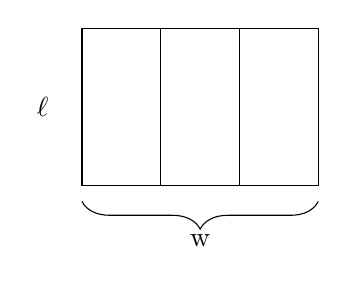
\begin{tikzpicture}
\draw (0,0)--(3,0)--(3,2)--(0,2)--(0,0) 
(1,0)--(1,2) (2,0)--(2,2);

\onslide<2->{\draw [decorate,decoration={brace,amplitude=10pt}]
(3,-.2) -- (0,-.2) node[xshift=1.5cm, yshift=-.5cm]{w}; 

\draw (-.5,1) node{$\ell$};}
\end{tikzpicture}
\end{center}
\only<3-|handout:0>{\color{answercolor}
The area is $A=\ell w$, and the amount of fencing gives us $4\ell+2w=1000$. Then $w=500-2\ell$, so 
\[A(\ell)=(500-2\ell)\ell=500\ell-2\ell^2\qquad
  A'(\ell)=500-4\ell\]

We differentiate to find CPs, and the maximum of $A$ over the domain $0 < \ell < 250$ is at $\ell=125$, which gives $w=250$ and $A=(125)(250)$ sq metres.
}
\end{frame}
%----------------------------------------------------------------------------------------
%----------------------------------------------------------------------------------------
\begin{frame}[t]
\note<1>{There are some nice arguments from symmetry that mean you can do this in your head}
\only<1>{\QuestionBar{3}{13}\AnswerYes}
\only<2>{\AnswerBar{3}{13}}
Suppose you want to make a rectangle with perimeter $400$. What dimensions give you the maximum area?
\pause\color{answercolor}\vfill

\answer{A 100-by-100 square.}
\end{frame}
%----------------------------------------------------------------------------------------
\begin{frame}[t]
\QuestionBar{4}{13}\AnswerYes

You are standing on the bank of a river that is 1km wide, and you want to reach the opposite side, two km down the river. You can paddle 3 kilometres per hour, and walk 6 kph while carrying your boat. What route takes you to your desired destination in the least amount of time? 
\vfill

\begin{tikzpicture}
\draw[C1, pattern=north west lines, pattern color=C1] (0,0)--(1,0)--(1,3)--(0,3)--cycle;

\draw (1,3) node[right]{ start};
\draw (0,0) node[left]{end };
\draw[M4, ultra thick, dashed] (1,3)--(1,1.5)--(0,0);
\draw (.5,3) node[above]{1};
\draw (0,1.5) node[left]{2};
\end{tikzpicture}
\vfill
\end{frame}
%----------------------------------------------------------------------------------------
\answer{\begin{frame}[t]
\AnswerBar{4}{13}
\color{answercolor}

Let $2-x$ be the distance you travel  carrying the boat, and then $\sqrt{x^2+1}$ is the distance you row. The time it takes is given by \[T(x)=\frac{1}{6}(2-x)+\frac{1}{3}\sqrt{x^2+1}\]
By differentiating, 
\[
T'(x)=-\frac{1}{6} + \frac{1}{3}\frac{x}{\sqrt{x^2+1}}
\]
we see the only critical point for positive $x$ is $x=\frac{1}{\sqrt{3}}$. This is the global minimum, so the fastest route is to portage (carry your boat) for $2-\frac{1}{\sqrt{3}}$ kilometres, then row the rest of the way. 
\end{frame}}
%----------------------------------------------------------------------------------------
%----------------------------------------------------------------------------------------
\begin{frame}[t]
\only<1>{\QuestionBar{5}{13}\AnswerYes}
\only<2>{\AnswerBar{5}{13}}
You are standing on the bank of a river that is 1km wide, and you want to reach the opposite side, two km down the river. You can paddle \textcolor{M4}{6} kilometres per hour, and walk \textcolor{M4}{3} kph while carrying your boat. What route takes you to your desired destination in the least amount of time? 

\vfill
\begin{tikzpicture}
\draw[C1, pattern=north west lines, pattern color=C1] (0,0)--(1,0)--(1,3)--(0,3)--cycle;

\draw (1,3) node[right]{ start};
\draw (0,0) node[left]{end };
\draw[M4, ultra thick, dashed] (1,3)--(1,1.5)--(0,0);
\draw (.5,3) node[above]{1};
\draw (0,1.5) node[left]{2};
\end{tikzpicture}
\pause\vfill\color{answercolor}

\answer{Paddle the whole way: it's faster, and more direct.}
\end{frame}
%----------------------------------------------------------------------------------------
%----------------------------------------------------------------------------------------
\begin{frame}[t]
\QuestionBar{6}{13}\AnswerYes\unote{Example~\eref{text}{APPglobalMaxMinDist}}

Let $C$ be the circle given by $x^2+y^2=1$. What is the closest point on $C$ to the point $(-2,1)$?
\vfill
\begin{center}\begin{tikzpicture}
\myaxis{x}{5}{2.25}{y}{2.25}{2.25}
\draw[C1, ultra thick] (0,0) node[shape=circle, inner sep=0, minimum size=4cm, draw]{};
\draw (-4,2) node[vertex]{};
\draw (-4,.2)--(-4,-.2) node[below]{$-2$};
\end{tikzpicture}\end{center}\vfill

\end{frame}
%----------------------------------------------------------------------------------------
\answer{\begin{frame}[t]
\AnswerBar{6}{13}
\color{answercolor}

We can reasonably see that the $y$-coordinate will be positive, and the $x$-coordinate negative. For any point $(x,y)$ on $C$, the distance $D$ to $(-2,1)$ is determined by:
\begin{align*}
D^2 &= \big(x-(-2)\big)^2+(y-1)^2\\
&= x^2+4x+4+\left(\sqrt{1-x^2} -1\right)^2\\
&=x^2+4x+4+(1-x^2)-2\sqrt{1-x^2}+1\\
&=4x+6-2\sqrt{1-x^2}
\end{align*}
where this only makes sense for $x$ between $-1$ and $1$. Minimizing $D$ is the same as minimizing $D^2$; so we take the derivative of the above function:
\[\diff{}{x}D(x)^2=4-2\frac{-2x}{2\sqrt{1-x^2}}
=4+\frac{2x}{\sqrt{1-x^2}}\] 
There are singular points at the endpoints $x= \pm 1$, and a critical point at $x=-\sqrt{4/5}$. Since $D(-1)^2=2$, $D(1)^2=10$, and
$D(-\sqrt{4/5})^2=6-\frac{10}{\sqrt{5}}\approx 1.53$, 
the closest point is \fbox{$(-\sqrt{4/5}, \sqrt{1/5})$}.
\end{frame}}
%----------------------------------------------------------------------------------------
%----------------------------------------------------------------------------------------
%----------------------------------------------------------------------------------------
\begin{frame}[t]
\only<1>{\QuestionBar{7}{13}\AnswerYes}
\only<2>{\AnswerBar{7}{13}}
Suppose you want to manufacture a closed cylindrical can on the cheap. If the can should have a volume of one litre (1000 cm$^3$), what is the smallest surface area it can have?\vfill

\pause
\answer{\color{answercolor}  Let the can have radius $r>0$ and height $h>0$. Then its volume is $1000=V=\pi r^2h$, and its surface area is 
$2(\pi r^2)+(2\pi r)h$. 

Using the volume equation, we know $h=\frac{1000}{\pi r^2}$, so for surface area, this gives us
\begin{align*}
S(r)&=2\pi r^2+2\pi r \frac{1000}{\pi r^2}
   = 2\pi r^2 + \frac{2000}{r} \\
S'(r)&=4\pi r - \frac{2000}{r^2}
      =4\pi r\left(1-\frac{500}{\pi r^3}\right)
\end{align*}
%We want the minimum value of $S$, so we find the critical and singular points.
%\[S'(r)=4\pi r - \frac{2000}{r^2}\]
The singular point $r=0$ is not in the domain of $S$; the only critical point is $r=\sqrt[3]{\frac{500}{\pi}}$. We see that, for $r$ smaller than the CP, 
$S'(r)<0$ so that $S(r)$ is decreasing, and that, for $r$ larger than the CP, $S'(r)>0$ so that $S(r)$ is increasing. 
So the minimum of $S(r)$ occurs at $r=\sqrt[3]{\frac{500}{\pi}}$ and 
\[
\text{minimum surface area }
=S\left(\sqrt[3]{\tfrac{500}{\pi}}\right)
=2\pi \left(\tfrac{500}{\pi} \right)^{2/3}+2000\left(\tfrac{\pi}{500}\right)^{1/3}\]}
\end{frame}
%----------------------------------------------------------------------------------------
%----------------------------------------------------------------------------------------
\begin{frame}[t]
\unote{Example~\eref{text}{APPglobalMaxMinB}}
\only<1>{\QuestionBar{8}{13}\AnswerYes}
\only<2>{\AnswerBar{8 }{13}}
 A cylindrical can is to hold 20$\pi$ cubic metres. The material for the top and bottom costs \$10 per square metre, and material for the side costs \$8 per square metre. Find the radius $r$ and height $h$ of the most economical can.\pause\color{answercolor}\vfill
 
\answer{The cost is $C = 8(2\pi rh)+2 \cdot 10 \cdot \pi r^2$. Since $20\pi=V =\pi r^2 h $, we see $rh = \frac{20}{r}$, so
\[C(r)=16\pi \frac{20}{r}+20\pi r^2\]
As
\[
C'(r) = 20\pi\left(-\frac{16}{r^2}+2r\right)
\]
$C(r)$ is minimized at $r=2$, and hence $h=5$.\vfill}
\end{frame}
%----------------------------------------------------------------------------------------

%----------------------------------------------------------------------------------------
%----------------------------------------------------------------------------------------

\begin{frame}[t]
\QuestionBar{9}{13}\AnswerYes
%\only<1-2>{\QuestionBar{9}{13}\AnswerYes}
Suppose a 2-metre high fence stands 1 metre away from a high wall. What is the shortest ladder that will reach over the fence to the wall?

\begin{center}
\begin{tikzpicture}
\draw (0,3)--(0,0)--(6,0);
\draw[M3, ultra thick] (1,0)--(1,2);
\draw[ultra thick, M5] (0,2.5)--(5,0);
\onslide<1>{\draw (-.2,1) node[rotate=90] {wall};
\draw[M3] (.8,1) node[rotate=90] {fence};
\draw[M5] (4,1) node{ladder};}

\onslide<2-|handout:0>{\draw (-.2,1) node {$y$};
\draw[M3] (.83,1) node {$2$};
\draw[M5] (2.7,1.5) node{$L$};
\draw [decorate,decoration={brace,amplitude=10pt}]
(5,-.2) -- (0,-.2) node[xshift=2.5cm, yshift=-.6cm]{x};
\draw (.5,.25) node{1};}
\end{tikzpicture}
\end{center}
\end{frame}
%----------------------------------------------------------------------------------------
\answer{\begin{frame}[t]
\AnswerBar{9}{13}
\color{answercolor}
\only<1|handout:0>{
To get $y$ in terms of $x$, we notice similar triangles tell us $\frac{y}{x} = \frac{2}{x-1}$, hence $y=\frac{2x}{x-1}$. The values of $x$ that make sense are $(1,\infty)$.


Noting $L^2=x^2+y^2=x^2+\frac{4x^2}{(x-1)^2}$, we see $L^2$ gets very large as $x$ gets close to 1 or as $x$ gets very large. As
\begin{align*}
\diff{}{x}L(x)^2&= 2x+\frac{8x}{(x-1)^2}-\frac{8x^2}{(x-1)^3} \\
&=2x(x-1)^3\big\{ (x-1)^3 +4(x-1) -4x\big\} \\
&=2x(x-1)^3\big\{ (x-1)^3 -4 \big\}
\end{align*}
the only critical point is at $x=\sqrt[3]{4}+1$, and this gives us our minimum 
$
L=
\sqrt{(\sqrt[3]{4}+1)^2+\dfrac{4(\sqrt[3]{4}+1)^2}{\sqrt[3]{4}^2}}
$.}

\end{frame}}
%----------------------------------------------------------------------------------------
%----------------------------------------------------------------------------------------
\begin{frame}[t]
\unote{Example~\eref{text}{APPglobalMaxMinrain}}
\QuestionBar{10}{13}\AnswerYes

Suppose a file folder is 12 inches long and 9 inches wide. You want to make a box by opening the folder and capping the ends. What angle should you open the folder to, to make the box with the greatest volume?
\vfill
\begin{center}
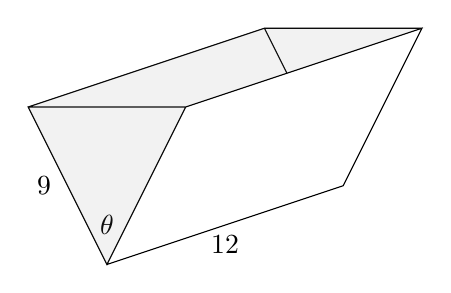
\begin{tikzpicture}
\draw (0,0)--(3,1)--(4,3)--(1,2)--(0,0)--(-1,2)--(1,2) (-1,2)--(2,3)--(4,3);
\draw (2,3)--(16/7,17/7);
\draw (-0.8,1) node{9};
\draw (1.5,.25) node{12};
\draw (0,.5) node{$\theta$};
\draw[fill=gray, opacity=.1] (-1,2)--(0,0)--(1,2)--(4,3)--(2,3)--(-1,2);
\end{tikzpicture}
\end{center}
\vfill
\end{frame}

%----------------------------------------------------------------------------------------

\answer{
\begin{frame}[t]
\AnswerBar{10}{13}
\color{answercolor}
The volume of a shape like this is the area of the triangular base, times the height, which is 12. So we maximize the volume by maximizing the area of the triangle with two sides of length 9, and angle between them $\theta$. 

This triangle has height $h=9\cos\frac{\theta}{2}$ 
              and base   $b=2\times 9\sin\frac{\theta}{2}$
 and so has area $\frac{1}{2}bh = 9^2\sin\frac{\theta}{2}\cos\frac{\theta}{2}
                                = \frac{9^2}{2}\sin \theta$. 

The maximum occurs at $\pi/2$. So, you want the folder to make a right angle.
\end{frame}
}
%----------------------------------------------------------------------------------------
%----------------------------------------------------------------------------------------
\begin{frame}[t]
\QuestionBar{11}{13}\AnswerYes
\begin{multicols}{2}
We want to bend a piece of wire into the perimeter of the shape shown below: a rectangle of height $h$ and width $2r$, with a half circle of radius $r$ on the top and bottom.
\vfill
If you only have 100cm of  wire, what values of $r$ and $h$ give the largest enclosed area?
\vfill
\columnbreak

\begin{center}
\begin{tikzpicture}
\draw(0,0) node[shape=circle, minimum size=3cm, inner sep=0, draw]{};
\draw(0,3) node[shape=circle, minimum size=3cm, inner sep=0, draw]{};
\draw[white, fill=white] (-1.5,0)--(-1.5,3)--(1.5,3)--(1.5,0)--(-1.5,0);
\draw (-1.5,0)--(-1.5,3) (1.5,3)--(1.5,0);
\draw[decorate,decoration={brace,
amplitude=10pt}] (-1.75,0)--(-1.75,3);
\draw (-2.5,1.55) node{$h$};

\draw[dashed] (-1.5,3)--(1.5,3)
 (-1.5,0)--(1.5,0);
\draw[decorate, decoration={brace, amplitude=10pt}] (1.5,3)--(0,3);
\draw (.75,2.25) node{$r$};
\end{tikzpicture}
\end{center}

\end{multicols}
\end{frame}
%----------------------------------------------------------------------------------------
%----------------------------------------------------------------------------------------
\begin{frame}<handout:0>[t]
\AnswerBar{11}{13}
\color{answercolor}
The perimeter is $100=2\pi r + 2h$, so
$h=50-\pi r$.

The area is
$\pi r^2 + 2rh = \pi r^2+2r(50-\pi r) =100r-\pi r^2=A(r)$.

\medskip 

As $A'(r)=100-2\pi r$, the maximum of $A(r)$ occurs at $r=\frac{50}{\pi}$. Then
$h=0$. That is: there's no rectangular part, only a circle.

\medskip

Circles are somehow more efficient at storing space than rectangles. More precisely, we mean that the ratio of area to perimeter is higher in circles 
than in rectangles. So the most efficient way to make the shape is to have the rectangular part have height 0.
\end{frame}
%----------------------------------------------------------------------------------------
%----------------------------------------------------------------------------------------
\begin{frame}[t]
\unote{Example~\eref{text}{APPglobalMaxMinE}}
\only<1>{\QuestionBar{12}{13}\AnswerYes}
\only<2>{\AnswerBar{12}{13}}
Suppose we take a right triangle, with height $h$ and base $b$. We inscribe a rectangle in it that shares a right angle, as shown below. What are the dimensions of the rectangle with the biggest area?

\begin{center}
\begin{tikzpicture}

\draw[very thick] (0,0)--(6,0)--(0,2)--(0,0);
\draw[M4, very thick] (0,1) -| (3,0);
\draw[M4, very thin, fill=M4, opacity=.1] (0,1) -| (3,0)-|(0,1);
\draw[decorate,decoration={brace, amplitude=10pt}, help lines] (6,-.2)--(0,-.2);
\draw (3,-1) node{$b$};

\draw[decorate,decoration={brace, amplitude=10pt}, help lines] (-.2,0)--(-.2,2);
\draw (-1,1) node{$h$};

\end{tikzpicture}
\end{center}
\answer{\vfill\pause\color{answercolor}
$b/2$ by $h/2$.}
\vfill
\end{frame}
%----------------------------------------------------------------------------------------
%----------------------------------------------------------------------------------------

%----------------------------------------------------------------------------------------
%----------------------------------------------------------------------------------------
\begin{frame}[t]{ACTIVITY}
\only<1>{\QuestionBar{13}{13}\AnswerNo}
By cutting out squares from the corners, turn a piece of paper into an open-topped box that holds a lot of beans.
\vfill
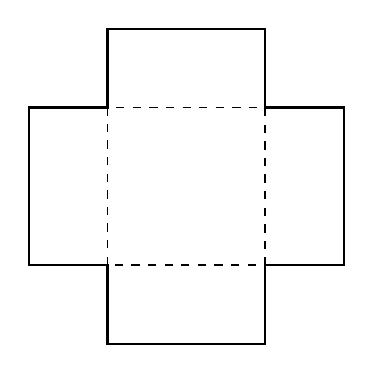
\begin{tikzpicture}
\draw[thick] (1,1)|-(3,0)|-(4,1)|-(3,3)|-(1,4)|-(0,3)|-cycle;
\draw[dashed] (1,1) rectangle (3,3);
\end{tikzpicture}
\unote{Example~\eref{text}{APPglobalMaxMinC}}
\note{I actually did this in class. It was pretty fun and it fits into about the last 15 minutes. I made bags of beans that fit in an optimal box, and students tried to make boxes that could fit them all. Almost every group got it. Bring paper, scissors, tape, rulers (printed on paper is fine), beans, and books.

Using printer paper, the boxes are not sturdy enough to fill with beans. I brought four big books to buttress the edges of each box as they were being filled. It turns out that boxes with really different dimensions from optimal can hold almost all the beans, which leads to another discussion: the curve at its maximum is fairly shallow, rather than steep.

You could probably do this without cutting: just fold the corners over. I haven't tried it that way. You could also give paper that had ruler marks printed on the four sides.}
\end{frame}
%----------------------------------------------------------------------------------------

